\section{Results}
\label{sec:results}

\subsection{Detection Benchmark}
\label{sec:detection}

Twelve architectures spanning two-stage, one-stage and query-based designs were trained on
the identical site-stratified split with identical preprocessing, which bounds how much of
the counting error any choice of backbone could account for.

\begin{table}[H]
\caption{\textbf{Detection on the held-out test split} (3725 images, 2792 boxes), 640\,px,
at confidence 0.25, ordered by F1; best per column in bold. AP$_{50}$ is the standard COCO
metric and the three F1 columns give the value under the stricter matching rules of
\cref{sec:criterion}; Precision, Recall, F1 and F$_{0.5}$ use the presence criterion. F1
rises monotonically as the rule relaxes, and centre-in-box tracks presence to within 0.032
for every model. The final column is the precision-weighted F-measure
$F_{0.5}=1.25\,PR/(0.25P+R)$, reported because the confirmation stage downstream is
constrained by precision rather than recall (\cref{sec:counting}); $\beta$ is fixed at the
conventional $0.5$ rather than tuned. Twelve architectures were trained; Deformable DETR R50
is excluded because its training ran out of GPU memory at epoch 5 (batch 8 on a 40\,GB
A100) and we did not pursue a smaller-batch rerun, so it is a resource limit on our side
rather than a result about the architecture.\label{tab:detectors}}
\begin{adjustwidth}{-\extralength}{0cm}
\centering\small
\begin{tabularx}{\fulllength}{lCCCCCCCC}
\toprule
\textbf{Model} & \textbf{AP$_\mathbf{50}$} & \textbf{F1 (IoU$\geq$.50)} & \textbf{F1 (IoU$\geq$.30)} & \textbf{F1 (Centre)} & \textbf{Precision} & \textbf{Recall} & \textbf{F1} & \textbf{F$_\mathbf{0.5}$} \\
\midrule
YOLOv8m & 0.459 & 0.502 & 0.603 & 0.628 & 0.780 & 0.572 & \textbf{0.660} & 0.727 \\
ATSS R50 & 0.380 & 0.441 & 0.556 & \textbf{0.648} & 0.683 & 0.635 & 0.658 & 0.673 \\
TOOD R50 & 0.396 & 0.442 & 0.572 & 0.623 & 0.683 & 0.621 & 0.650 & 0.670 \\
YOLO11m & 0.460 & \textbf{0.535} & \textbf{0.623} & 0.638 & 0.897 & 0.503 & 0.645 & \textbf{0.775} \\
RT-DETR-L & 0.434 & 0.497 & 0.595 & 0.610 & 0.643 & 0.605 & 0.623 & 0.635 \\
YOLO12m & 0.508 & 0.506 & 0.583 & 0.595 & \textbf{0.929} & 0.452 & 0.608 & 0.767 \\
YOLOv9m & 0.506 & 0.527 & 0.581 & 0.592 & 0.917 & 0.450 & 0.604 & 0.759 \\
YOLOv10m & \textbf{0.510} & 0.527 & 0.575 & 0.583 & 0.874 & 0.453 & 0.597 & 0.737 \\
DINO R50 & 0.365 & 0.425 & 0.520 & 0.548 & 0.560 & 0.572 & 0.566 & 0.562 \\
Faster R-CNN R50 & 0.418 & 0.376 & 0.475 & 0.497 & 0.393 & 0.723 & 0.509 & 0.433 \\
RTMDet-m & 0.466 & 0.339 & 0.411 & 0.437 & 0.325 & \textbf{0.779} & 0.459 & 0.368 \\
\bottomrule
\end{tabularx}
\end{adjustwidth}
\end{table}

\Cref{tab:detectors} shows first how little separates them: AP$_{50}$ spans 0.365--0.510,
with the top three within 0.004, across designs as different as Faster R-CNN, DINO and
YOLO12m. That narrow spread is the signature of a data-limited rather than an
architecture-limited regime, and \cref{fig:training} shows it is not an artefact of any
model being under-trained: within the budget each run either plateaus or passes its peak,
and the plateaus sit on top of one another. The one genuinely unsettled curve is DINO R50,
which is still oscillating between 0.15 and 0.30 mAP@50 at the point its budget expires ---
the slow convergence the query-based literature reports, visible directly.

The absolute values are low for two reasons, neither of them a model failure. The first is
geometric: for axis-aligned boxes of side $s$ offset by $d$ pixels,
$\mathrm{IoU}=(s-d)/(s+d)$, so at the corpus median $s=27$ a four-pixel centre error already
fails a 0.75 threshold and nine pixels fails 0.50. Scoring at strict IoU demands sub-pixel
localization on animals 27 pixels across with diffuse thermal boundaries. The second is that
these metrics count boxes rather than animals: an animal visible for 100 frames contributes
100 ground-truth boxes, and one found in half of them scores 0.5 recall even though counting
requires a single detection. The 11,476 background frames contribute nothing either way,
since precision, recall and F1 have no true-negative term. Counted per animal, the same
detectors that score around 0.50 box recall find 220 of the 235 annotated deer in at least
one frame, and the full pipeline reaches 82 of 83 on held-out video (\cref{sec:counting}).
The distance between 0.50 and 0.94 is not a discrepancy but two metrics answering different
questions --- the first sign that detection accuracy is a poor proxy for counting ability.

A third pattern belongs to individual rows rather than to the table as a whole, and it is
what makes an entry like YOLO12m's 0.929 precision against 0.452 recall look
self-contradictory. It is not. The two numbers describe one conservative operating point:
of YOLO12m's errors at confidence 0.25, 1530 are missed boxes and 96 are false ones, so
\textbf{94\% of its error is silence rather than mistake}. A model that is quiet is not a
model that is wrong, and the distinction matters downstream, because the two failures cost
the confirmation stage very different amounts.

\begin{table}[H]
\caption{\textbf{The precision--recall split is a threshold choice, not a capability
limit.} The two strongest detectors of \cref{tab:detectors}, scored on the same test split
under the presence criterion, at the conventional reporting threshold of 0.25 and at the
0.10 the counting pipeline actually runs the detector at. Rows are ordered by the best F1
either threshold achieves. That ordering is for reading, not a verdict: F1 weights
precision and recall equally, which \cref{sec:choosing} argues is the wrong balance for a
counting pipeline, and under the precision-weighted $F_{0.5}$ we actually select on,
YOLO11m leads at 0.775 against YOLO12m's 0.767. Lowering the threshold buys YOLO12m 20
points of recall for 22 of precision, which is one knob on one curve. The direction of the
trade matters more than its size, because it is not symmetric, and the lower rows show it:
a detector already operating at high recall has nowhere left to go. Dropping RT-DETR-L to
0.10 buys 231 additional true boxes and costs 7433 false ones, collapsing precision to
0.187 --- not a candidate pool any confirmation stage can work with, which is the argument
of \cref{sec:inversion} appearing one stage earlier.\label{tab:threshold}}
\centering\small
\setlength{\tabcolsep}{3pt}
\begin{tabularx}{\textwidth}{lCCCCCCC}
\toprule
\textbf{Model} & \textbf{Conf.} & \textbf{Precision} & \textbf{Recall} & \textbf{F1} & \textbf{TP} & \textbf{FP} & \textbf{FN} \\
\midrule
\multirow{2}{*}{YOLO12m} & 0.25 & \textbf{0.929} & 0.452 & 0.608 & 1262 & \textbf{96} & 1530 \\
 & 0.10 & 0.711 & \textbf{0.653} & \textbf{0.681} & 1824 & 741 & \textbf{968} \\
\midrule
\multirow{2}{*}{YOLO11m} & 0.25 & 0.897 & 0.503 & 0.644 & 1404 & 162 & 1388 \\
 & 0.10 & 0.777 & 0.576 & 0.661 & 1608 & 462 & 1184 \\
\bottomrule
\end{tabularx}
\end{table}

\Cref{tab:threshold} gives the sensitivity. At 0.10 the same YOLO12m weights score 0.711
precision and 0.653 recall, so the low recall in \cref{tab:detectors} is a property of the
reporting threshold rather than of the model. This also means the figure in
\cref{tab:detectors} is not the operating point of the system this paper describes:
\textbf{the counting pipeline runs the detector at confidence 0.10}, where recall is 20
points higher, and 0.25 is reported only because it is the conventional threshold for a
detection table. Recall is further understated by the matching rule --- relaxing IoU$\geq$0.50
to presence cuts YOLO12m's false positives from 307 to 96 while its misses fall only from
1741 to 1530, because a looser criterion can credit a box that was placed a few pixels off
an animal but cannot recover an animal the detector never fired on.

\begin{figure}[H]
\begin{adjustwidth}{-\extralength}{0cm}
  \centering
  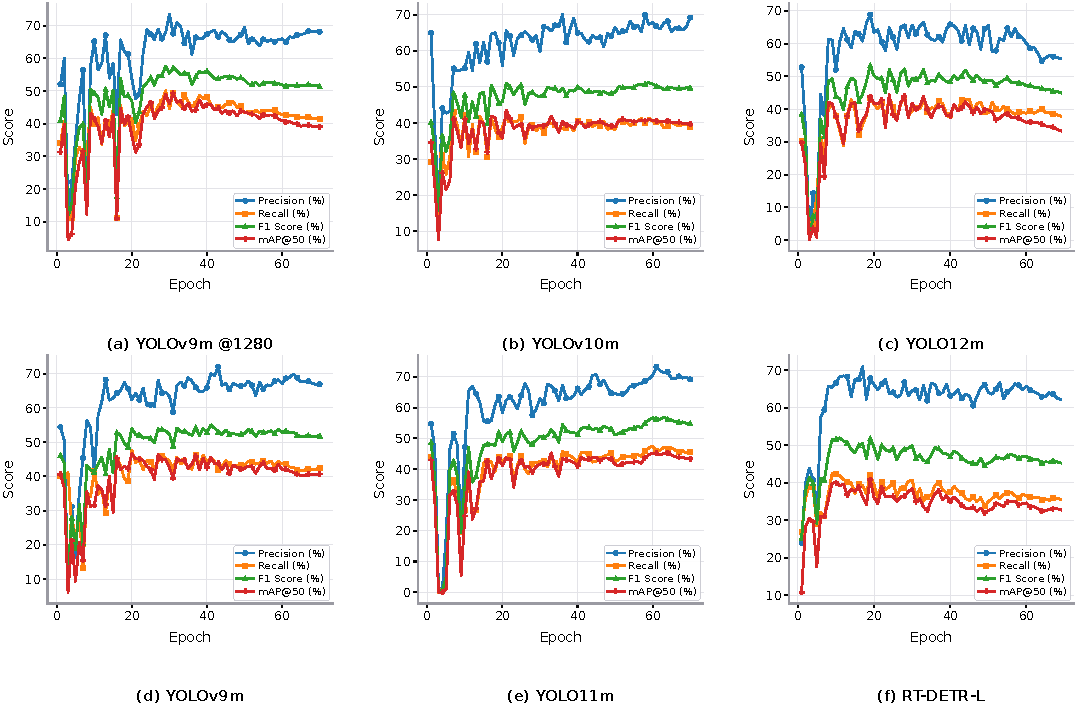
\includegraphics[width=\fulllength]{figures/fig5_training.pdf}
\end{adjustwidth}
  \caption{\textbf{Validation curves for every architecture in \cref{tab:detectors}.} One
  panel per detector, drawn from the training logs each run wrote; no curve is smoothed or
  re-fitted. The two frameworks record different quantities, so the series differ by family
  and each panel carries its own legend: the Ultralytics models (\textbf{a}--\textbf{g})
  log precision, recall and mAP@50 per epoch, from which F1 is computed, while the
  mmdetection models (\textbf{h}--\textbf{l}) log the COCO mAP family. Epoch counts differ by
  framework rather than by budget: the Ultralytics runs stop on a patience criterion,
  while the mmdetection runs complete fixed schedules of 70 epochs, or 36 for DINO's
  native schedule, validating every second epoch. The $y$-axes are not shared.
  Two patterns matter for what follows. Precision settles near 0.65--0.70 while recall
  settles near 0.40--0.45 in every Ultralytics panel, which is the operating point
  \cref{sec:choosing} argues the counting stage actually needs; and several models
  (\textbf{c}, \textbf{f}, \textbf{i}) peak early and then decline, so the reported figures
  come from the best checkpoint rather than the last. Deformable DETR R50 is absent because its
  training ran out of GPU memory at epoch 5, so it has no curve to draw
  (\cref{tab:detectors}).\label{fig:training}}
\end{figure}

One architectural pattern survives every criterion. The query-based detectors underperform:
DINO R50 reaches 0.365 AP$_{50}$ on a full native schedule, below plain Faster R-CNN, and
Deformable DETR did not converge within budget. RT-DETR-L, which targets that weakness,
recovers to 0.434 but still trails the convolutional one-stage models.

\subsection{Choosing a Detector for Counting}
\label{sec:choosing}

\begin{figure}[H]
  \centering
  
\includegraphics[width=0.8\linewidth]{figures/fig3_criterion.pdf}
  \caption{\textbf{Rank under IoU$\geq$0.50 does not predict rank under the counting
  criterion.} Seven of eleven models shift by two or more places; YOLOv10m falls from 2nd to
  8th. Choosing a detector for a counting system by its detection metric selects the wrong
  model.\label{fig:criterion}}
\end{figure}

The narrow spread in aggregate scores conceals a substantial difference in operating point.
YOLO12m and YOLOv9m sit at 0.929 and 0.917 precision against roughly 0.45 recall, while
RTMDet-m and Faster R-CNN R50 occupy the opposite end, reaching 0.779 and 0.723 recall at
0.33 and 0.39 precision. Since a matching criterion determines how errors of each type are
counted, rank depends on which criterion is applied. \Cref{fig:criterion} plots the shift:
seven of eleven models move at least two places, YOLOv10m falls from 2nd to 8th, and ATSS
R50 climbs from 8th to 2nd. Selecting a detector on its detection metric does not select the
model that counts best.

Both AP$_{50}$ and F1 weight precision and recall equally, which does not reflect the cost
structure of the stage that consumes these detections. The confirmation step must reject
tens of thousands of false candidates against roughly two hundred true ones
(\cref{sec:counting}), so a false positive and a false negative are not equally expensive to
it, and \cref{sec:inversion} shows that enlarging the candidate pool degrades the final
count rather than improving it. We therefore summarize with the precision-weighted
$F_{0.5}$ in the last column of \cref{tab:detectors}, fixing $\beta$ at its conventional
value rather than selecting it. YOLO11m ranks first at 0.775, ahead of YOLO12m at 0.767 and
YOLOv9m at 0.759. That margin of 0.008 makes the top three effectively equivalent; the
substantive separation is from the recall-oriented models at 0.368--0.433. We adopt
\textbf{YOLO11m at 640\,px} as the production detector, and every counting result in this
paper uses it.

\begin{table}[H]
\caption{\textbf{640 versus 1280\,px.} Higher resolution helps YOLOv9m on every column and
hurts YOLOv10m on every column: at 640 the two are within 0.004 AP$_{50}$, at 1280 they
diverge by 0.047. AP-small moves the other way for both (0.128 to 0.119 and 0.117 to 0.093),
so the small-object deficit is not primarily a resolution deficit.\label{tab:resolution}}
\centering
\begin{tabularx}{\textwidth}{lCCCCC}
\toprule
\textbf{Model} & \textbf{Resolution} & \textbf{Precision} & \textbf{Recall} & \textbf{F1} & \textbf{AP$_\mathbf{50}$} \\
\midrule
YOLOv9m & 640 & 0.704 & 0.448 & 0.547 & 0.506 \\
\textbf{YOLOv9m} & \textbf{1280} & \textbf{0.757} & \textbf{0.491} & \textbf{0.595} & \textbf{0.516} \\
YOLOv10m & 640 & 0.674 & 0.455 & 0.543 & 0.510 \\
YOLOv10m & 1280 & 0.669 & 0.432 & 0.525 & 0.469 \\
\bottomrule
\end{tabularx}
\end{table}

Resolution is the one lever that behaves unpredictably. \Cref{tab:resolution} shows
1280\,px helping YOLOv9m on every metric and hurting YOLOv10m on every one; at 640 the two
are within 0.004 AP$_{50}$, at 1280 they diverge by 0.047. AP-small falls for both, so the
extra resolution buys overall precision and recall rather than the smallest animals.

That gain does not survive the pipeline. YOLOv9m at 1280\,px is the strongest detector in
this section by AP$_{50}$ (0.516 against YOLO11m's 0.460), so we ran it through the complete
counting pipeline under the protocol of \cref{sec:heldout}. It counts \emph{fewer} animals:
MAE 2.54 and 54 of 83 held-out animals, against 2.38 and 55 of 83 for YOLO11m at 640\,px.
A 12\% advantage in detection accuracy becomes a small deficit in counting accuracy, which
is why the production detector is not the one this section ranks highest, and the first
direct evidence for the divergence the rest of the paper characterizes.

\subsection{End-to-End Counting}
\label{sec:counting}

\begin{table}[H]
\caption{\textbf{End-to-end counting.} The held-out row is the honest number: the rule is
swept on the 19 detector-training videos, frozen, and applied to the 13 held-out ones. Bias
is consistently negative --- the system under-counts and essentially never over-counts, which
is the conservative direction for a wildlife survey.\label{tab:counting}}
\centering
\begin{tabularx}{\textwidth}{lCCC}
\toprule
\textbf{Scope} & \textbf{MAE} & \textbf{Bias} & \textbf{Counted} \\
\midrule
Fit videos (detector trained on these) & 1.53 & $-0.05$ & 99.3\% \\
\textbf{Held out (13 videos)} & \textbf{2.38} & $\mathbf{-1.92}$ & \textbf{66.3\%} \\
All 32 videos (optimistic) & 1.88 & $-0.81$ & 89.0\% \\
\bottomrule
\end{tabularx}
\end{table}

\Cref{tab:counting} is the end-to-end result: \textbf{MAE 2.38 animals per video and 66.3\%
of held-out animals counted}, with a bias of $-1.92$. The system under-counts systematically
and over-counts almost never, which for management purposes is the safe direction --- a
survey that never inflates its estimate is preferable to one that occasionally does.

\begin{table}[H]
\caption{\textbf{Per-video breakdown on the 13 held-out videos.} GT is the annotated number
of individual animals; Reach and Prim.\ are the decomposition of \cref{sec:decomposition};
Count is the number the pipeline reports and Err its signed error. Reading a row left to
right attributes that video's loss to a stage. NShelbyRd loses 5 animals to detection
(27$\to$22) and a further 6 to association (22$\to$16), the largest tracking failure in the
corpus and the reason dense-group video dominates the error. GolfDr and SIron are the only
videos that over-count, and both do so while their reach and primary counts are complete ---
the error there is confirmation accepting spurious tracks, not missing
animals.\label{tab:pervideo}}
\centering
\begin{tabularx}{\textwidth}{llRRRRR}
\toprule
\textbf{Video} & \textbf{Site} & \textbf{GT} & \textbf{Reach} & \textbf{Prim.} & \textbf{Count} & \textbf{Err} \\
\midrule
NShelbyRd (blue) & SHB & 27 & 22 & 16 & 20 & $-7$ \\
GolfDr & SHB & 12 & 12 & 10 & 14 & $+2$ \\
NWolfCreek (orange) & SHB & 9 & 9 & 9 & 5 & $-4$ \\
GiantCityRd & TON & 8 & 7 & 7 & 3 & $-5$ \\
Robinson & SHW & 7 & 7 & 7 & 7 & $0$ \\
Melvin & SHW & 5 & 5 & 5 & 1 & $-4$ \\
AquaCultureRd & TON & 3 & 1 & 1 & 0 & $-3$ \\
N25thBlue & MAS & 3 & 3 & 3 & 3 & $0$ \\
NMarseilles & MAS & 3 & 3 & 3 & 1 & $-2$ \\
OikosRd & TON & 2 & 2 & 2 & 1 & $-1$ \\
TouchofNature & TON & 2 & 1 & 1 & 0 & $-2$ \\
ChipsRd & TON & 1 & 1 & 1 & 1 & $0$ \\
SIron & SHW & 1 & 1 & 1 & 2 & $+1$ \\
\midrule
\textbf{Total} & & \textbf{83} & \textbf{74} & \textbf{66} & \textbf{58} & $\mathbf{-25}$ \\
\bottomrule
\end{tabularx}
\end{table}

\Cref{tab:pervideo} gives the breakdown per video, and reading a row left to right
attributes that video's loss to a stage. The error concentrates in dense-group footage: SHB
contributes 9 of the 25 net missing animals from three videos, and its group-heavy NShelbyRd
transect alone accounts for 7, losing 5 animals to detection and a further 6 to association.
Only two videos over-count, and both do so with complete reach and primary counts, so their
error is confirmation accepting spurious tracks rather than anything upstream.

Under the stricter identity-matched criterion of \cref{sec:decomposition} --- animals
covered by an \emph{accepted} track, rather than per-video count agreement --- the figure is
47/83 = 56.6\%. The 10-point gap is coincidental agreement: accepted tracks that do not land
on an animal offsetting animals that were missed. The capped aggregate is our headline
figure, for comparability with the counting literature; the identity-matched figure is
reported alongside it because the two answer different questions.

\subsection{Improving Candidate Generation Makes Counting Worse}
\label{sec:inversion}

This is the paper's central experimental result. We improved the candidate pool four
independent ways and measured the effect on the decomposition and on the final count.

\begin{figure}[H]
  \centering
  
\includegraphics[width=0.8\linewidth]{figures/fig2_inversion.pdf}
  \caption{\textbf{The inversion.} As candidate generation improves, more animals become
  reachable and fewer are counted. Both series are animals out of 83 and share one
  axis.\label{fig:inversion}}
\end{figure}

\begin{table}[H]
\caption{\textbf{Every improvement to candidate generation degrades the count.} Pool G
reaches 82 of 83 held-out animals and gives 73 their own track --- the best pool we built, at
less than a third of pool F's candidate count --- yet counts fewer animals than pool C, which
reaches only 74. ``Ceiling'' is \primaryq/83, the maximum a one-count-per-track confirmation
stage could achieve. \reachedq and \primaryq are counted per animal; \countedq is the
per-video capped aggregate defined in \cref{sec:decomposition}, which is the figure the
counting literature reports. Its per-animal equivalent is lower --- 47, 47, 37 and 47
respectively.\label{tab:pools}}
\begin{adjustwidth}{-\extralength}{0cm}
\centering\footnotesize
\setlength{\tabcolsep}{4pt}
\begin{tabular}{llrccccc}
\toprule
\textbf{Pool} & \textbf{Intervention} & \textbf{Candidates} & \textbf{\reachedq} & \textbf{\primaryq} & \textbf{\countedq} & \textbf{MAE} & \textbf{Ceiling} \\
\midrule
C & Orphan recovery, conf 0.10 (operating point) & 7008 & 74/83 & 66/83 & \textbf{55/83 = 66.3\%} & \textbf{2.38} & 79.5\% \\
E & \quad + track-init gate removed, conf 0.02 & 18,349 & 79/83 & 69/83 & 54/83 = 65.1\% & 2.54 & 83.1\% \\
F & \quad + NMS IoU $0.50\!\to\!0.90$ & 90,239 & 79/83 & 70/83 & 41/83 = 49.4\% & 3.46 & 84.3\% \\
G & \quad + appearance re-identification & 27,679 & \textbf{82/83 = 98.8\%} & \textbf{73/83 = 88.0\%} & 52/83 = 62.7\% & 2.69 & \textbf{88.0\%} \\
\bottomrule
\end{tabular}
\end{adjustwidth}
\end{table}

\Cref{tab:pools} and \cref{fig:inversion} give the result, one row per intervention. Each
does what it was designed to do:

\begin{itemize}[leftmargin=*,labelsep=4.5mm]
\item \textbf{Lowering detector confidence} 0.10$\to$0.02 and \textbf{removing the tracker's
track-ini\-tial\-i\-za\-tion gate} raised \reachedq from 74 to 79. Lowering confidence \emph{alone}
recovered zero additional animals: the gate, not the threshold, was the binding constraint
--- BoT-SORT will extend a track from a low-confidence detection but will not \emph{start}
one, so faint animals were invisible to counting regardless of detector threshold.
\item \textbf{Loosening NMS} to IoU 0.90 addressed animals standing close enough that one
box suppressed another; it added 4 \primaryq at the cost of $5\times$ the candidates.
\item \textbf{Appearance re-identification} produced the best pool by every measure: 82 of
83 animals reached, 73 with their own track, at 27,679 candidates --- fewer than a third of
pool F's for four more \primaryq. It genuinely works: it merges fragments of one animal
rather than merely adding candidates.
\end{itemize}

And the count falls, monotonically in candidate volume: 55, 54, 52, 41. The confirmation
stage cannot exploit a pool it did not shrink. Each intervention adds far more negatives
than positives --- pool G has 219 positive tracks against 27,460 negatives --- and a
three-parameter rule tuned to survive that ratio must be aggressive enough to reject real
animals along with the noise.

\subsection{Pipeline Ablations}
\label{sec:ablations}

\begin{table}[H]
\caption{\textbf{Pipeline ablation, held out on the 13 videos the detector never trained
on.} Each row changes one stage of the full pipeline in the first row; all other stages are
held fixed. The pattern is uniform and is the paper's central result: \emph{no change to
detection, tracking or association improves the count}. Appearance re-identification
produces the best candidate pool by a wide margin --- 82 of 83 animals reached and 73 given
their own track, at less than a third of the loose-NMS candidate volume --- and still counts
three fewer animals than the baseline. The only row that changes the confirmation stage is
also the only place where a substantial loss appears without a corresponding pool change,
and \cref{tab:confirmers} expands that comparison across four methods and two
pools.\label{tab:ablationmain}}
\begin{adjustwidth}{-\extralength}{0cm}
\centering\footnotesize
\setlength{\tabcolsep}{4pt}
\begin{tabular}{llrrrrr}
\toprule
\textbf{Stage} & \textbf{Configuration} & \textbf{Candidates} & \textbf{\reachedq} & \textbf{\primaryq} & \textbf{\countedq} & \textbf{MAE} \\
\midrule
--- & \textbf{Full pipeline} (YOLO11m@640, orphans, 3-param rule) & 7008 & 74/83 & 66/83 & \textbf{55/83} & \textbf{2.38} \\
\midrule
Detection & \quad detector $\to$ YOLOv9m @1280\,px (best AP$_{50}$) & 1496 & 67/83 & 62/83 & 54/83 & 2.54 \\
Tracking & \quad $-$ orphan recovery & 711 & 66/83 & 59/83 & 52/83 & 2.46 \\
Tracking & \quad $+$ track-init gate removed, conf 0.02 & 18,349 & 79/83 & 69/83 & 54/83 & 2.54 \\
Detection & \quad $+$ NMS IoU $0.50 \to 0.90$ & 90,239 & 79/83 & 70/83 & 41/83 & 3.46 \\
Association & \quad $+$ appearance re-identification & 27,679 & \textbf{82/83} & \textbf{73/83} & 52/83 & 2.69 \\
Confirmation & \quad rule $\to$ temporal transformer & 7008 & 74/83 & 66/83 & 49/83 & 2.85 \\
\bottomrule
\end{tabular}
\end{adjustwidth}
\end{table}

\begin{figure}[H]
\begin{adjustwidth}{-\extralength}{0cm}
  \centering
  
\includegraphics[width=\fulllength]{figures/qualitative.png}
\end{adjustwidth}
  \caption{\textbf{Tracking through overlap and low contrast, on held-out video.} Four frames
  from three transects the detector never trained on. Box colour encodes track identity and
  is stable over time; each label gives the track ID and its calibrated per-track score.
  \textbf{Top row:} the same scene 0.3\,s apart, five animals tracked and five counted in
  both frames. Tracks 3035 and 3041 retain their identities across the pair while the camera
  translates beneath them, and the animals at the right of the frame stand close enough that
  their boxes overlap without their identities merging. \textbf{Bottom left:} a fourfold
  range spread inside one frame, from a near animal at 87\,px to a distant one at 22\,px;
  the per-track score falls with range, so the confidence reports the difficulty rather than
  concealing it. \textbf{Bottom right:} two animals of 42 and 50\,px against a near-uniform
  thermal background, overlapping in image space and individually close to indistinguishable,
  are still carried as two tracks. Overlap and low contrast are the two conditions under
  which a counting system silently merges individuals into one, and neither does so
  here.\label{fig:qualitative}}
\end{figure}

\Cref{tab:ablationmain} gives the pipeline ablation with one stage changed per row. One entry
from the wider set is worth isolating: lowering detector confidence from 0.10 to 0.05 added
3807 candidates and recovered \emph{zero} additional animals, which ruled out the detector
threshold and pointed us at the tracker's initialization gate.

\Cref{fig:qualitative} shows what the association stage does on held-out video under the two
conditions that make counting fail. The first is overlap. When two animals stand close
enough that their boxes intersect, a tracker that leans on spatial proximity will hand both
to one identity, and the pair is counted once; the top row and the bottom-right frame each
contain such a pair, and in both the animals are carried as separate tracks with separate
identities. The second is low contrast. In the bottom-right frame the animals are a few tens
of pixels across against an almost uniform thermal field, close to the point where a human
reader would hesitate to call them animals at all, and they are still tracked. Persistence
is visible directly in the top row: the two frames are 0.3\,s apart, the whole scene
translates between them as the vehicle moves, and the identities survive the translation
because motion compensation removes the camera's contribution before association. The
bottom-left frame shows the range spread a single transect frame can contain --- 87\,px and
22\,px animals simultaneously --- with the calibrated score falling as the animal recedes,
which is the behaviour a per-track posterior is meant to have.

\subsection{What the Confidence Condition Buys}
\label{sec:sensitivity}

The confirmation rule's three parameters are hand-set, and the confidence condition
$c\ge0.65$ is the one a reader is most likely to challenge. The detector did find those
animals; discarding a candidate because its five best frames average below 0.65 looks like
throwing away recall that was already paid for. This subsection measures exactly that, and
the answer is more interesting than a threshold defence: the condition is not a recall
filter at all.

\begin{table}[H]
\caption{\textbf{Deleting the confidence condition, all else fixed.} The published operating
point ($m\ge20$, $s\ge0$) is held and only $c$ moves; every column is the 13 held-out videos,
83 animals. Lowering $c$ recovers real animals --- coverage rises 23 points --- and admits
duplicates faster, so the system passes through approximate unbiasedness at $c\approx0.45$
and ends over-counting by 28 animals at $c=0$. The published $c=0.65$ minimizes MAE; it does
not maximize coverage, and \cref{sec:discussion} argues that for a survey this is the right
trade.\label{tab:confsens}}
\centering
\begin{tabularx}{\textwidth}{CCCCCCC}
\toprule
\textbf{$c$} & \textbf{Predicted} & \textbf{Counted} & \textbf{MAE} & \textbf{Bias} & \textbf{Over} & \textbf{Under} \\
\midrule
0.00 & 111 & \textbf{89.2\%} & 3.54 & $+2.15$ & 37 & 9 \\
0.15 & 111 & \textbf{89.2\%} & 3.54 & $+2.15$ & 37 & 9 \\
0.25 & 108 & 85.5\% & 3.77 & $+1.92$ & 37 & 12 \\
0.35 &  99 & 80.7\% & 3.69 & $+1.23$ & 32 & 16 \\
0.45 &  81 & 72.3\% & 3.38 & $\mathbf{-0.15}$ & 21 & 23 \\
0.55 &  70 & 71.1\% & 2.69 & $-1.00$ & 11 & 24 \\
\textbf{0.65} & \textbf{58} & 66.3\% & \textbf{2.38} & $-1.92$ & 3 & 28 \\
0.75 &  24 & 28.9\% & 4.54 & $-4.54$ & 0 & 59 \\
0.85 &   0 &  0.0\% & 6.38 & $-6.38$ & 0 & 83 \\
\bottomrule
\end{tabularx}
\end{table}

\Cref{tab:confsens} holds the other two parameters at their published values and moves only
$c$. Three things follow.

First, \textbf{the objection is half right}. Removing the condition entirely raises held-out
coverage from 66.3\% to 89.2\%. That is the largest coverage gain produced by any single
change in this paper --- larger than all four candidate-generation interventions of
\cref{sec:inversion}, none of which raised coverage at all. Those animals really were being
discarded, and they really do come back.

Second, \textbf{they do not come back alone}. The pipeline predicts 111 animals where 83
exist. Over-counts rise from 3 to 37 while under-counts fall only from 28 to 9, so MAE
degrades from 2.38 to 3.54 and the bias flips from $-1.92$ to $+2.15$. In animals: 53
additional tracks are accepted, of which 19 are animals that were previously missed and 34
are not, so the pipeline buys each recovered animal at the price of roughly two duplicates.

Third, and this is the substantive point, \textbf{the condition is a duplicate suppressor
rather than a detector threshold}. A fragment sitting on an animal that has already been
counted is a true detection --- an animal really is there --- so nothing in the question
``is this a deer?'' separates it from a first sighting. Sustained high confidence across a
track is the cheapest signal available that does separate them, because a duplicate fragment
is typically short and weakly scored where the animal's primary track is neither. That is
why $c$ cannot be relaxed to recover recall: recall and duplicate suppression are being
bought with the same parameter.

A practical corollary is visible in the bias column. The MAE-optimal setting is deliberately
conservative, under-counting by 1.9 animals per video. A survey that needs an approximately
\emph{unbiased} estimator rather than a minimum-error one should set $c\approx0.45$, where
the bias is $-0.15$, and accept 1.0 more MAE for it. We report the MAE-optimal rule as the
headline because it is the conventional choice, but which of the two a practitioner wants
depends on whether their downstream statistic is sensitive to variance or to bias.

\begin{table}[H]
\caption{\textbf{The same question, with the other two parameters free.} For each $c$ the
grid search re-fits $m$ and $s$ on the 19 detector-training videos, so $c$ is never
handicapped by a stale companion setting; the rule is then frozen and reported on the 13
held-out videos. Given the freedom to compensate, the sweep responds to a lowered $c$ by
tightening the span constraint instead --- buying precision with duration --- and the
substitution is a poor one: coverage lands \emph{below} the frozen variant of
\cref{tab:confsens}, because a one-second minimum discards short tracks belonging to real
animals.\label{tab:confsensrefit}}
\centering
\begin{tabularx}{\textwidth}{CCCCCC}
\toprule
\textbf{$c$} & \textbf{Fitted $m$} & \textbf{Fitted $s$ (s)} & \textbf{Fit MAE} & \textbf{Held-Out MAE} & \textbf{Held-Out Counted} \\
\midrule
0.00 & 20 & 1.0 & 3.47 & 3.69 & 60.2\% \\
0.15 & 20 & 1.0 & 3.42 & 3.69 & 60.2\% \\
0.25 & 20 & 1.0 & 3.21 & 3.69 & 60.2\% \\
0.35 &  5 & 1.0 & 3.11 & 4.00 & 56.6\% \\
0.45 & 20 & 0.5 & 3.05 & 3.85 & 60.2\% \\
0.55 & 20 & 0.5 & 2.42 & 3.31 & 59.0\% \\
\textbf{0.65} & \textbf{20} & \textbf{0.0} & \textbf{1.53} & \textbf{2.38} & \textbf{66.3\%} \\
0.75 &  1 & 0.0 & 4.16 & 4.31 & 32.5\% \\
0.85 &  1 & 0.0 & 7.89 & 6.38 & 0.0\% \\
\bottomrule
\end{tabularx}
\end{table}

\Cref{tab:confsensrefit} repeats the experiment with $m$ and $s$ re-fitted for each $c$, so
that the confidence condition is not blamed for a companion parameter left at a stale value.
The conclusion strengthens. Across the full $7\times6\times9=378$-cell grid, only two values
of $c$ --- 0.55 and 0.65 --- appear among the twelve best cells by fit MAE, and the three best
are the same $c=0.65$ rule with the span parameter at 0, 0.1 and 0.25. The span parameter is
therefore \emph{inert} at the operating point: three different values give identical fits,
so the published rule is effectively two parameters wearing a third. We keep the third
because it is what the sweep uses to compensate when $c$ is lowered, which is precisely the
behaviour this table is designed to expose.

\subsection{The Rule Is Not the Bottleneck}
\label{sec:learned}

\Cref{sec:sensitivity} shows the rule's parameters are load-bearing rather than arbitrary.
The remaining question is whether the \emph{form} of the rule is what limits the count. If
so, replacing it with a learned confirmer should help. We tested that under three protocols
and it does not.

\begin{table}[H]
\caption{\textbf{Held-out confirmation comparison.} All methods trained and thresholded on
the 19 detector-training videos, reported on the 13 held out. Learned confirmers lose on
pool C and tie on pool G. Logistic regression on pool G fails in the opposite direction,
predicting 102 animals where 83 exist.\label{tab:confirmers}}
\centering
\begin{tabularx}{\textwidth}{llCC}
\toprule
\textbf{Pool} & \textbf{Confirmer} & \textbf{MAE} & \textbf{Counted} \\
\midrule
\multirow{4}{*}{C} & \textbf{Hand-tuned rule (3 params)} & \textbf{2.38} & \textbf{55/83} \\
 & Gradient boosting & 2.85 & --- \\
 & Logistic regression & 3.00 & --- \\
 & Temporal transformer ($\sim$60k params) & 2.85 & 49/83 \\
\midrule
\multirow{4}{*}{G} & Hand-tuned rule & 2.77 & 50/83 \\
 & Gradient boosting & 2.92 & --- \\
 & Logistic regression & 3.15 & --- \\
 & Temporal transformer & 2.77 & 51/83 \\
\bottomrule
\end{tabularx}
\end{table}

\Cref{tab:confirmers} gives the held-out comparison. Every learned method loses on pool C ---
gradient boosting and the temporal transformer both at 2.85 MAE, logistic regression at
3.00, against the rule's 2.38 --- and on the richer pool G the transformer only ties, at
2.77. Every learned variant \emph{under-counts harder} than the rule, indicating that they
reject additional candidates rather than recovering the animals the rule discards.

Two further protocols agree. Under 8-fold cross-validation over videos the rule again wins
(1.88 MAE), and the pattern across that sweep is diagnostic: performance degrades
monotonically with model capacity --- logistic regression at 13 parameters reaches 3.41,
gradient boosting at $10^3$ reaches 2.41--2.66, and the transformer at $6\times10^4$ reaches
2.81 --- while shrinking a gradient-boosted model to depth-1 stumps ($\sim$40 effective
parameters) recovers nearly the whole gap and achieves the best RMSE of any method. This is
a variance limit, not an architectural one.

We also trained directly on the counting objective, letting fragments share probability mass
so the loss is $|\sum_i p_i - c|$ rather than per-track cross-entropy. It was the worst
variant tested, which rules out ``the rule wins because it optimizes MAE directly'' as the
explanation.

Having established \emph{where} the animals are lost, we ask \emph{which} animals and why.

\subsection{Which Animals Are Missed}
\label{sec:analysis}

\begin{figure}[H]
  \centering
  
\includegraphics[width=0.8\linewidth]{figures/fig4_scale.pdf}
  \caption{\textbf{A hole in the training distribution.} The training split contains no box
  above 96\,px. Three missed animals sit at 104, 149 and 157\,px --- one of them never
  detected at all. A detector that finds 27\,px animals does not miss a 149\,px one unless it
  has never seen one.\label{fig:scale}}
\end{figure}

Of the 83 held-out animals, the detector never fires on 9 (median 20\,px, at the sensor's
limit) and the rule rejects 27 that it did find. Of those 27, \textbf{26 fail the confidence
condition} and one fails purely on track length: their five best detections average below
0.65, though five do reach 0.65 in a single frame, so the failure is one of sustained rather
than peak confidence. Those 26 are the entire remaining opportunity ---
though \cref{sec:sensitivity} shows they cannot be recovered by moving the threshold that
rejects them, since doing so admits roughly two duplicates for each. We verified by direct
inspection that none of the 36 are annotation errors --- each was rendered with its
ground-truth box at three points in its track --- and all are real animals.

\begin{table}[H]
\caption{\textbf{Fate of the 83 held-out animals.} The detector finds 74 of 83; the
confirmation rule then discards 27 of them. Missed animals are smaller and shorter-lived
than counted ones, and the rejected group sits \emph{between} the other two on every measure
--- which is precisely why a threshold on any single one of them cannot separate
it.\label{tab:missed}}
\centering
\begin{tabularx}{\textwidth}{lRRRR}
\toprule
\textbf{Outcome} & \textbf{$n$} & \textbf{Median Box} & \textbf{GT Frames} & \textbf{Cand.\ Conf.} \\
\midrule
Counted & 47 & 38.1\,px & 102 & 0.76 \\
\textbf{Rejected by the rule} & \textbf{27} & 28.0\,px & 47 & 0.52 \\
Never detected & 9 & 19.9\,px & 47 & --- \\
\bottomrule
\end{tabularx}
\end{table}

\Cref{tab:missed} gives the per-group statistics behind that split, and the ordering in the
final column is the reason \cref{sec:learned} finds what it finds: the rejected group sits
between the counted and undetected groups on box size, track length and candidate
confidence alike, so no threshold on any one of them separates it cleanly.

That inspection produced an unexpected finding. Three of the missed animals are not small but
very \emph{large}: 104, 149 and 157\,px against a corpus median of 27, and the 149\,px animal
was never detected at all. \Cref{fig:scale} gives the likely explanation: the largest
training box is 95.6\,px and the split contains \emph{zero} boxes at or above 100\,px, so all
three sit outside the annotated size distribution. Scale augmentation does present enlarged
copies, so the detector is not strictly naive to large objects, but enlargement is sampled
rarely while mosaic augmentation shrinks objects concurrently. The mirror image of the
small-object problem is visible here: the detector performs worst where examples are
scarcest.

The obvious remedy is to widen scale augmentation until the training distribution reaches
100--200\,px, and we report here that we have not yet established whether it works. Two
earlier attempts appeared to collapse to near-zero mAP within three epochs, and we
attributed that to the symmetry of the standard implementation: sampling from
$[1-m,\,1+m]$ means that reaching $2.2\times$ also means sampling $0\times$, which drives a
27\,px animal to sub-pixel size on a corpus that is 71\% small objects. That attribution
was wrong, and so was the premise behind it. Both runs were cancelled after five and ten
minutes of wall-clock respectively; neither diverged. What they recorded --- mAP@50 of
0.406, 0.138 and 0.001 across their first three epochs --- is the ordinary transient of this
training recipe, not a failure of it. The baseline detector, trained with the standard
symmetric setting, passes through the same trough: 0.429, 0.299, 0.000, 0.000, 0.010, and
then 0.316 by its sixth epoch, before going on to the result in \cref{tab:detectors}. The
dip coincides with the end of the three-epoch learning-rate warm-up and it resolves without
intervention. Read against that curve, the two aborted runs were on an unremarkable
trajectory when they were stopped.

Two further corrections belong here, because both bear on how reproducible this remedy is.
Asymmetric scaling is \emph{not} absent from common frameworks: Ultralytics accepts an
explicit $(\mathrm{lo},\mathrm{hi})$ pair from version 8.4, so enlarging the upper tail
without touching the lower one needs a configuration change rather than new code. And
mosaic augmentation does not shrink objects --- the implementation composes a $2\times$
canvas and crops it back to the input size, so object pixel dimensions are preserved, and
the interaction we had described between mosaic and scale does not exist. We therefore make
no claim in either direction about whether widening the scale distribution helps: the
experiment that would settle it, holding every other hyperparameter at the baseline's
values and moving only the sampling bounds, is the one that should be run, and reporting an
untested mechanism in its place would be worse than reporting nothing.

The loss is concentrated regardless of the remedy: the one video containing these animals
counts 3 of 8, three of its five misses being the oversized individuals, so this is worth
roughly 4 points of the headline figure.

\subsection{Individual Re-Identification at 27 Pixels}
\label{sec:reid}

\begin{table}[H]
\caption{\textbf{Re-identification is dominated by size, not appearance.} All cues scored on
the same 69 held-out animals. A two-number size descriptor reaches 0.638 and an ImageNet
backbone scores \emph{below} plain geometry. The trained encoder's 0.899 is largely range
matching, not identity. It is a probe for how much identity signal the imagery carries, not
a component of the counting system: the appearance term in the pipeline uses the detector's
own backbone features.\label{tab:reid}}
\centering
\begin{tabularx}{\textwidth}{lC}
\toprule
\textbf{Cue} & \textbf{Rank-1} \\
\midrule
Chance & 0.101 \\
Mean intensity alone & 0.101 \\
Thermal silhouette alone (scale removed) & 0.435 \\
Raw thermal crop & 0.493 \\
\textbf{Box size alone ($w,h$)} & \textbf{0.638} \\
ImageNet ResNet-50 features & 0.725 \\
Geometry (size, aspect, intensity) & 0.797 \\
Trained thermal encoder & \textbf{0.899} \\
\bottomrule
\end{tabularx}
\end{table}

A natural proposal for the association stage is appearance-based individual
re-identification. Because the annotation gives one track per individual, the corpus already
contains identity labels and the question can be settled empirically. We evaluate closed-set
re-identification on \textbf{69 animals in 7 videos the detector never trained on}: each
track is split temporally, the first half forms the gallery and the second half the query.
Within video is the \emph{ceiling}, since both halves share range, pose and thermal
calibration, so a low score is decisive.

A trained thermal encoder reaches rank-1 0.899 (\cref{tab:reid}), which sounds like working
re-identification until the decomposition. \textbf{Box size alone reaches 0.638}, and within
a video an animal's range changes slowly, so most of what looks like identification is
matching \emph{distance}. Appearance in isolation is weak: mean intensity carries exactly
chance information, silhouette with scale removed reaches 0.435, and a pretrained CNN lands
below plain geometry. At a median $29\times24$ pixels there is not enough detail to key an
identity to, so we describe the system as performing \emph{track association} --- preventing
double counting within a survey --- and make no individual-identification claim. Appearance
does help the \emph{association} stage, which is a far easier problem: enabling it gives the
best candidate pool in the paper, 82 of 83 animals reached and 73 given their own track
(\cref{tab:ablationmain}). That pool still counts three fewer animals than the baseline,
so better association does not translate into a better count --- the same pattern every other
pool improvement follows.
